\documentclass{article}

% Language setting
% Replace `english' with e.g. `spanish' to change the document language
\usepackage[russian]{babel}

% Set page size and margins
% Replace `letterpaper' with `a4paper' for UK/EU standard size
\usepackage[a4paper,top=2cm,bottom=2cm,left=3cm,right=3cm,marginparwidth=1.75cm]{geometry}

% Useful packages
\usepackage{amsmath, amssymb, amsthm}
\usepackage{indentfirst}
\usepackage{graphicx, float}
\usepackage[colorlinks=true, allcolors=blue]{hyperref}

\newcommand{\argmin}{\arg\!\min}
\newcommand{\argmax}{\arg\!\max}

\setlength{\parskip}{5pt}
\setlength{\parindent}{20pt}
\title{Эмпирические байесовские нейронные сети}
\author{Басов Дмитрий Константинович}
\date{}
\begin{document}
\maketitle

\begin{abstract}
Данная статья посвящена применению техники эмпирического Байеса к байесовским нейронным сетям. Концептуально идея следующая:
\begin{enumerate}
 \item Мы используем диагональное нормальное распределение для аппроксимации апостериорного распределения весов модели~--- $q(W)$.
 \item Априорное распределение весов модели так же задаётся диагональным распределением с нулевым матожиданием~--- $p(W)$.
 \item Используя вариационный вывод, мы приходим к ситуации, когда ELBO зависит от $KL(q(W)~||~p(W))$. Так как оба распределения являются нормальными, то KL дивергенция считается аналитически.
 \item Мотивация следующего этапа была взята из RVM~--- взять дисперсию априорного распределения весов модели $p(W)$ из данных. Там несложно берётся производная и всё получается красиво, кроме возможного деления 0/0. Но сделав замену переменных, от этой беды можно уйти.
\end{enumerate}
Пункты 1--3 в принципе были описаны в статье \href{https://arxiv.org/pdf/1505.05424}{Weight Uncertainty in Neural Networks}. А вот четвёртый пункт я ни в книгах, ни в статьях не находил.
\end{abstract}


\section{Обозначения и сокращения}
$N(\mu, \sigma^2)$ --- нормальное распределение

$\pmb{x} \odot \pmb{y}$ --- поэлементное произведение (произведение Адамара) векторов

$\mathcal{L}$ --- Evidence Lower Bound (ELBO)

$KL(q~||~p) = \int_{}{} q(\pmb{Z}) \cdot \ln{\dfrac{q(\pmb{Z})}{p(\pmb{Z})}} d \pmb{Z}$ --- дивергенция Кульбака--Лейблера

$\pmb{x}$ --- вектор признаков

$\pmb{y}$ --- вектор целевой переменной

$D$ --- датасет --- пары значений \{$\pmb{x_i}$, $\pmb{y_i}$\}, где $i = 1, \dots, L$

$\pmb{W}$ --- веса модели --- случайная величина размерности M

$p(D | \pmb{W}) = \prod_{i=1}^{L} p(\pmb{y_i} | \pmb{x_i}, \pmb{W})$ — правдоподобие (likelihood)

$p(\pmb{W})$ --- априорное распределение весов модели (prior)

$p(\pmb{W}| D)$ --- апостериорное распределение весов модели (posterior)

$p(D)$ --- маргинальная вероятность датасета (evidence)

$
p(\pmb{W}, D) =
p(D | \pmb{W}) \cdot p(\pmb{W}) =
p(\pmb{W}| D)\cdot p(D)
$ --- совместная вероятность весов модели и данных

$q(\pmb{W} | \pmb{\theta})$ --- аппроксимация апостериорного распределения весов модели

$\pmb{\theta}$ --- обучаемые параметры байесовской модели

\section{Введение}

В классическом машинном обучении делается следующее предположение: веса модели $\pmb{W}$ являются пусть и неизвестной, но фиксированной величиной. В этом случае можно получить точечную оценку весов модели согласно гипотезе максимального правдоподобия.

\[
\pmb{W_{ML}} = \argmax_{\pmb{W}} p(D | \pmb{W})
\]

Тогда распределение $p(\pmb{y} | \pmb{x}, D)$ аппроксимируется следующим образом:

\[
p(\pmb{y} | \pmb{x}, D) \approx p(\pmb{y} | \pmb{x}, \pmb{W_{ML}})
\]

Однако это справедливо при условии, что количество объектов в датасете D сильно больше количества весов модели ($L \gg M$). Если это не так, веса модели $\pmb{W}$ могут слишком сильно подстроиться под обучающую выборку D, что черевато переобучением.

Для борьбы с переобучением используется ряд приёмов (штрафы на норму весов, early stopping, dropout), однако для их настройки требуются вычислительные ресурсы и отложенные (не участвующие в обучении) выборки данных.

Альтернативным подходом к машинному обучению является нахождение апостериорного распределения весов модели $p(\pmb{W}| D)$ по теореме Байеса.

\[
p(\pmb{W}| D) =
\dfrac{p(D | \pmb{W}) \cdot p(\pmb{W})}{\int_{}{} p(D | \pmb{W}) \cdot p(\pmb{W}) d \pmb{W}}
\]

Тогда предсказательное распределение $p(\pmb{y} | \pmb{x}, D)$ рассчитывается следующим образом:

\[
p(\pmb{y} | \pmb{x}, D) =
\int_{}{} p(\pmb{y} | \pmb{x}, \pmb{W}) \cdot p(\pmb{W} | D) d \pmb{W}
\approx \dfrac{1}{T} \sum_{t=1}^{T}{p(\pmb{y} | \pmb{x}, \hat{\pmb{W}}_{p(\pmb{W} | D)_{t}})}
\]
где $\hat{\pmb{W}}_{p(\pmb{W} | D)_{t}}$ --- сэмпл весов модели из $p(\pmb{W}| D)$.

Байесовские модели машинного обучения можно рассматривать как ансамбль из бесконечного числа моделей, веса которых сэмплируются из распределения $p(\pmb{W}| D)$. Такой подход устойчив к переобучению, так как о размере обучающей выборки не делается никаких предположений. Однако возникают следующие проблемы: выбор подходящего априорного распределения $p(\pmb{W})$ и вычисление апостериорного распределения $p(\pmb{W}| D)$.

Неудачный выбор $p(\pmb{W})$ может сильно ухудшить качество модели, а расчёт апостериорного распределения $p(\pmb{W}| D)$ требует вычисления интеграла по всему пространству весов модели, что для нейронных сетей практически невозможно.

В данной статье предлагается следующий подход к решению этих проблем.

\begin{enumerate}
 \item Вместо распределения $p(\pmb{W}| D)$ используется его аппроксимация $q(\pmb{W} | \pmb{\theta})$. Используя технику вариационного вывода, задача сводится к максимизации нижней вариационной границы (ELBO) $\mathcal{L}(q(\pmb{W} | \pmb{\theta}))$ по параметрам $\pmb{\theta}$.
 \item Распределение $q(\pmb{W} | \pmb{\theta})$ задаётся в виде нормального распределения с диагональной матрицей ковариации. То есть каждый вес модели определяется двумя числами, которые определяют его математическое ожидание и дисперсию. Таким образом, количество обучаемых параметров относительно классической нейронной сети возрастает в 2 раза.
 \item Априорное распределение весов модели $p(\pmb{W})$ задаётся в виде нормального распределения с нулевым матожиданием (из соображений симметрии) и диагональной матрицей ковариации. То есть мы вносим следующее априорное знание: веса модели находятся около нуля.
 \item Для определения дисперсии априорного распределения весов модели $p(\pmb{W})$ применяется техника эмпирического Байеса. То есть значение дисперсии $p(\pmb{W})$ берётся из датасета D. Так как распределения $q(\pmb{W} | \pmb{\theta})$ и $p(\pmb{W})$ являются нормальными, оптимальное значение дисперсии распределения $p(\pmb{W})$ определяется аналитически. Такой подход обладает большой универсальностью, однако из--за этого теряется теоретическая устойчивость к переобучению.
 \item Так как распределение $q(\pmb{W} | \pmb{\theta})$ является нормальным, применяя трюк с репараметризацией, становится возможным использовать градиентные методы для максимизации $\mathcal{L}(q(\pmb{W} | \pmb{\theta}))$.
 \item Вводятся новые параметры $\pmb{\gamma}$ и $\pmb{\rho}$, через которые выражаются матожидание и дисперсия распределения $q(\pmb{W} | \pmb{\theta})$. Это нужно, чтобы избежать неопределенности деления $\dfrac{0}{0}$, которая может возникнуть из--за определения дисперсии распределения $p(\pmb{W})$ из данных.
\end{enumerate}

Эксперименты показали, что предлагаемый подход сохраняет гибкость классических нейронных сетей и делает их устойчивыми к переобучению.

\section{Постановка задачи}

Задача машинного обучения с учителем в вероятностной постановке формулируется следующим образом: получить распределение вероятностей $p(\pmb{y} | \pmb{x}, D)$ целевой переменной $\pmb{y}$ для неразмеченных $\pmb{x}$, используя информацию из датасета D. В случае параметрические моделей, которыми являются нейронные сети, информация из датасета D кодируется посредством весов модели $\pmb{W}$. Сделаем следующие преобразования:

\[
p(\pmb{y} | \pmb{x}, D) =
\int_{}{} p(\pmb{y}, \pmb{W} | \pmb{x}, D) d \pmb{W} =
\int_{}{} p(\pmb{y} | \pmb{W}, \pmb{x}, D) \cdot p(\pmb{W} | \pmb{x}, D) d \pmb{W} =
\int_{}{} p(\pmb{y} | \pmb{W}, \pmb{x}) \cdot p(\pmb{W} | D) d \pmb{W}
\]

Пояснения:
\begin{itemize}
 \item $p(\pmb{y} | \pmb{x}, D) = \int_{}{} p(\pmb{y}, \pmb{W} | \pmb{x}, D) d \pmb{W}$, так как для любых случайных величин $\pmb{a}$ и $\pmb{b}$ справедливо $p(\pmb{a}) = \int p(\pmb{a}, \pmb{b}) d \pmb{b}$
 \item $p(\pmb{y}, \pmb{W} | \pmb{x}, D) = p(\pmb{y} | \pmb{W}, \pmb{x}, D) \cdot p(\pmb{W} | \pmb{x}, D)$, так как для любых случайных величин $\pmb{a}$ и $\pmb{b}$ справедливо $p(\pmb{a}, \pmb{b}) = p(\pmb{a}| \pmb{b}) \cdot p(\pmb{b})$
 \item $p(\pmb{y} | \pmb{W}, \pmb{x}, D) = p(\pmb{y} | \pmb{W}, \pmb{x})$, так как вся информация из датасета D отражена в весах $\pmb{W}$
 \item $p(\pmb{W} | \pmb{x}, D) = p(\pmb{W} | D)$, так как веса модели $\pmb{W}$ не зависят от неразмеченных $\pmb{x}$, которых не было в датасете D.
\end{itemize}

Получим выражение для $p(\pmb{W}| D)$, используя формулу Байеса:

\[
p(\pmb{W}| D) =
\dfrac{p(\pmb{W}, D)}{p(D)} =
\dfrac{p(\pmb{W}, D)}{\int_{}{} p(\pmb{W}, D) d \pmb{W}} =
\dfrac{p(D | \pmb{W}) \cdot p(\pmb{W})}{\int_{}{} p(D | \pmb{W}) \cdot p(\pmb{W}) d \pmb{W}}
\]

Для аппроксимации распределения ответов модели можно воспользоваться методом Монте--Карло. Идея следующая: cэмплируем конечное количество весов $\hat{\pmb{W_1}}, \dots, \hat{\pmb{W_T}}$ из распределения $p(\pmb{W}| D)$  и аппроксимируем распределение $p(\pmb{y} | \pmb{x}, D)$ следующим образом:

\[
p(\pmb{y} | \pmb{x}, D)
\approx \dfrac{1}{T} \sum_{t=1}^{T}{p(\pmb{y} | \pmb{x}, \hat{\pmb{W}}_{p(\pmb{W} | D)_{t}})}
\]
где $\hat{\pmb{W}}_{p(\pmb{W} | D)_{t}}$ --- сэмпл весов модели из $p(\pmb{W}| D)$.

Однако для этого нужно иметь возможность сэмплировать из распределения $p(\pmb{W}| D)$. Получить аналитическое решение интеграла $\int_{}{} p(D | \pmb{W}) \cdot p(\pmb{W}) d \pmb{W}$ можно только в очень ограниченном числе случаев.

Существует возможность сэмплировать из $p(\pmb{W}| D)$, используя методы Монте--Карло для марковских цепей (MCMC). Однако для больших датасетов и большого числа весов это практически невозможно.

Альтернативным подходом к решению такой задачи является вариационный вывод --- аппроксимация распределения $p(\pmb{W}| D)$ распределением $q(\pmb{W} | \pmb{\theta})$, из которого сэмплировать намного проще.

\section{Вариационный вывод}

Идея вариационного вывода --- сведение задачи байесовского вывода к задаче максимизации нижней вариационной границы (ELBO) $\mathcal{L}$, которая для распределения $q(\pmb{W} | \pmb{\theta})$ записывается следующим образом:

\[
\mathcal{L}(q(\pmb{W} | \pmb{\theta})) =
\int_{}{} q(\pmb{W} | \pmb{\theta}) \cdot \ln{\dfrac{p(\pmb{W}, D)}{q(\pmb{W} | \pmb{\theta})}} d \pmb{W}
\]

В этом случае аппроксимация предсказательного распределения $p(\pmb{y} | \pmb{x}, D)$ будет выглядить следующим образом:

\[
p(\pmb{y} | \pmb{x}, D)
\approx \dfrac{1}{T} \sum_{t=1}^{T}{p(\pmb{y} | \pmb{x}, \hat{\pmb{W}}_{q(\pmb{W} | \pmb{\theta})_{t}})}
\]
где $\hat{\pmb{W}}_{q(\pmb{W} | \pmb{\theta})_{t}}$ --- сэмпл весов модели из $q(\pmb{W} | \pmb{\theta})$.

Покажем мотивацию максимизации ELBO. Запишем выражение для $KL(q(\pmb{W} | \pmb{\theta})~||~p(\pmb{W}| D))$ и преобразуем его, используя тождество $p(\pmb{W}, D) = p(\pmb{W}| D)\cdot p(D)$:

\[
KL(q(\pmb{W} | \pmb{\theta})~||~p(\pmb{W}| D)) =
\int_{}{} q(\pmb{W} | \pmb{\theta}) \cdot \ln{\dfrac{q(\pmb{W} | \pmb{\theta})}{p(\pmb{W}| D)}} d \pmb{W} =
\int_{}{} q(\pmb{W} | \pmb{\theta}) \cdot \ln{\dfrac{p(D) \cdot q(\pmb{W} | \pmb{\theta})}{p(\pmb{W}, D)}} d \pmb{W} =
\]\[
\ln{p(D)} \cdot \int_{}{} q(\pmb{W} | \pmb{\theta}) d \pmb{W} - \int_{}{} q(\pmb{W} | \pmb{\theta}) \cdot \ln{\dfrac{p(\pmb{W}, D)}{q(\pmb{W} | \pmb{\theta})}} d \pmb{W} =
\ln{p(D)} - \mathcal{L}(q(\pmb{W} | \pmb{\theta}))
\]

Так как $\ln{p(D)}$ не зависит от $\pmb{\theta}$, максимизация $\mathcal{L}(q(\pmb{W} | \pmb{\theta}))$ по параметрам $\pmb{\theta}$ ведёт к минимизации $KL(q(\pmb{W} | \pmb{\theta})~||~p(\pmb{W}| D))$. Тем самым, при максимизации $\mathcal{L}(q(\pmb{W} | \pmb{\theta}))$ распределение $q(\pmb{W} | \pmb{\theta})$ будет приближаться к распределению $p(\pmb{W}| D)$.

Преобразуем выражение для $\mathcal{L}(q(\pmb{W} | \pmb{\theta}))$, используя тождество $p(\pmb{W}, D) = p(D | \pmb{W}) \cdot p(\pmb{W})$:

\[
\mathcal{L}(q(\pmb{W} | \pmb{\theta})) =
\int_{}{} q(\pmb{W} | \pmb{\theta}) \cdot \ln{\dfrac{p(\pmb{W}, D)}{q(\pmb{W} | \pmb{\theta})}} d \pmb{W} =
\int_{}{} q(\pmb{W} | \pmb{\theta}) \cdot \ln{\dfrac{p(D | \pmb{W}) \cdot p(\pmb{W})}{q(\pmb{W} | \pmb{\theta})}} d \pmb{W} =
\]\[
\int_{}{} q(\pmb{W} | \pmb{\theta}) \cdot \ln{p(D | \pmb{W})} d \pmb{W} - \int_{}{} q(\pmb{W} | \pmb{\theta}) \cdot \ln{\dfrac{q(\pmb{W} | \pmb{\theta})}{p(\pmb{W})}} d \pmb{W} =
\]\[
\int_{}{} q(\pmb{W} | \pmb{\theta}) \cdot \ln{p(D | \pmb{W})} d \pmb{W} - KL(q(\pmb{W} | \pmb{\theta})~||~p(\pmb{W})) =
\]\[
\int_{}{} q(\pmb{W} | \pmb{\theta}) \cdot \sum_{i=0}^{L} {\ln{p(\pmb{y_{i}} | \pmb{x_{i}}, \pmb{W})}} d \pmb{W} - KL(q(\pmb{W} | \pmb{\theta})~||~p(\pmb{W}))
\]

Таким образом, выражение для $\mathcal{L}(q(\pmb{W} | \pmb{\theta}))$ раскладывается на два слагаемых. Первое слагаемое показывает, насколько хорошо распределение $q(\pmb{W} | \pmb{\theta})$ описывает датасет D. Второе слагаемое показывает, насколько хорошо распределение $q(\pmb{W} | \pmb{\theta})$ соответствует распределению $p(\pmb{W})$.

\section{Задание функциональных форм распределений}
Для дальнейшнего вывода положим, что распределения $p(\pmb{W})$ и $q(\pmb{W} | \pmb{\theta})$ являются нормальными с диагональными матрицами ковариации:

$
p(\pmb{W}) =
N(\pmb{W} | \pmb{0}, diag(\pmb{\sigma_{p(\pmb{W})}})^{2})$,
где $\pmb{\sigma_{p(\pmb{W})}}$ — вектор длины M

$q(\pmb{W} | \pmb{\theta}) = N(\pmb{W} | \pmb{\mu}, diag(\pmb{\sigma_{q(\pmb{W})}})^{2})$, где $\pmb{\mu}$ и $\pmb{\sigma_{q(\pmb{W})}}$ — вектора длины M, которые вместе образуют вектор обучаемых параметров $\pmb{\theta}$.

Априорное распределение весов модели $p(\pmb{W})$ имеет нулевое математическое ожидание (из соображений симметрии), и среднеквадратическое отклонение $\pmb{\sigma_{p(\pmb{W})}}$. В классическом байесовском выводе параметр $\pmb{\sigma_{p(\pmb{W})}}$ должен задаваться до начала обучения, то есть являться гиперпараметром. Однако мы можем воспользоваться техникой эмпирического Байеса, то есть определить параметр  априорного распределения $\pmb{\sigma_{p(\pmb{W})}}$ из данных.

Пусть $\pmb{\alpha} = diag(\pmb{\sigma_{p(\pmb{W})}})^{-2}$. Тогда
$
p(\pmb{W}) =
N(\pmb{W} | \pmb{0}, \pmb{\alpha}^{-1})$
.

Так как распределения $p(\pmb{W})$ и $q(\pmb{W} | \pmb{\theta})$ являются нормальными, то $KL(q(\pmb{W} | \pmb{\theta})~||~p(\pmb{W}))$ можно посчитать аналитически:

\[
KL(q(\pmb{W} | \pmb{\theta})~||~p(\pmb{W})) =
\dfrac{1}{2}\sum_{k=1}^{M}(\dfrac{\sigma_{{q(W)_{k}}}^2}{\sigma_{{p(W)_{k}}}^2} + \dfrac{\mu_{k}^2}{\sigma_{{p(W)_{k}}}^2} - \ln{\dfrac{\sigma_{{q(W)_{k}}}^2}{\sigma_{{p(W)_{k}}}^2}} - 1) =
\]\[
\dfrac{1}{2}\sum_{k=1}^{M}(\alpha_k (\sigma_{{q(W)_{k}}}^2 + \mu_{k}^2) - \ln{(\alpha_k \cdot \sigma_{{q(W)_{k}}}^2)} - 1)
\]

Так как в выражении
$\mathcal{L}(q(\pmb{W} | \pmb{\theta}))$
интеграл
$\int_{}{} q(\pmb{W} | \pmb{\theta}) \cdot \ln{p(D | \pmb{W})} d \pmb{W}$
не зависит от параметров распределения $p(\pmb{W})$, то:

\[
\dfrac{\partial \mathcal{L}(q(\pmb{W} | \pmb{\theta}))}{\partial {\alpha_k}} =
- \dfrac{\partial (KL(q(\pmb{W} | \pmb{\theta})~||~p(\pmb{W})))}{\partial {\alpha_k}} =
-\dfrac{1}{2}(\sigma_{{q(W)_{k}}}^2 + \mu_{k}^2 - \dfrac{1}{\alpha_k}) =
-\dfrac{1}{2}(\sigma_{{q(W)_{k}}}^2 + \mu_{k}^2 - \sigma_{{p(W)_{k}}}^2)
\]

Приравняв производную к нулю, получим:

\[
-\dfrac{1}{2}(\sigma_{{q(W)_{k}}}^2 + \mu_{k}^2 - \sigma_{{p(W)_{k}}}^2) = 0
\]
\[
\sigma_{{p(W)_{k}}}^2 = \sigma_{{q(W)_{k}}}^2 + \mu_{k}^2
\]

Подставив полученное выражение в $KL(q(\pmb{W} | \pmb{\theta})~||~p(\pmb{W}))$, получим:

\[
KL(q(\pmb{W} | \pmb{\theta})~||~p(\pmb{W})) =
\dfrac{1}{2}\sum_{k=1}^{M}\ln({1 + \dfrac{\mu_{k}^2}{\sigma_{{q(W)_{k}}}^2}})
\]
\[
\mathcal{L}(q(\pmb{W} | \pmb{\mu}, \pmb{\sigma_{q(\pmb{W})}})) =
\int_{}{} q(\pmb{W} | \pmb{\mu}, \pmb{\sigma_{q(\pmb{W})}}) \cdot \ln{p(D | \pmb{W})} d \pmb{W} - \dfrac{1}{2}\sum_{k=1}^{M}\ln({1 + \dfrac{\mu_{k}^2}{\sigma_{{q(W)_{k}}}^2}})
\]

\section{Замена переменных}

При максимизации $\mathcal{L}(q(\pmb{W} | \pmb{\mu}, \pmb{\sigma_{q(\pmb{W})}}))$ могут возникнуть ситуации, когда какой--либо вес модели перестает быть случайной величиной и вырождается в ноль ($\sigma_{{q(W)_{k}}} \rightarrow 0$ и $\mu_{k} \rightarrow 0$). Это приведет к неопределенности деления 0 на 0 при вычислении KL--дивергенции. Чтобы избежать этой неопределенности, и чтобы $\pmb{\sigma_{q(\pmb{W})}}$ была всегда положительна, сделаем следующую замену переменных:

$\sigma_{{q(W)_{k}}} = \ln({1 + e^{\rho_{k}}}) = Softplus(\rho_{k})$

$\mu_{k} = \gamma_{k} \cdot Softplus(\rho_{k})$

Тогда:

\[
KL(q(\pmb{W} | \pmb{\theta})~||~p(\pmb{W})) =
\dfrac{1}{2}\sum_{k=1}^{M}\ln({1 + \dfrac{\mu_{k}^2}{\sigma_{{q(W)_{k}}}^2}}) =
\dfrac{1}{2}\sum_{k=1}^{M}\ln({1 + \gamma_{k}^{2}})
\]

Таким образом, задача сводится к минимизации следующей функции потерь:

\[
Loss(\pmb{\rho}, \pmb{\gamma}) =
- \dfrac{\mathcal{L}(q(\pmb{W} | \pmb{\theta}))}{L} =
\int_{}{} N(\pmb{W} | \pmb{\mu}, diag(\pmb{\sigma_{q(\pmb{W})}})^{2}) \cdot NLL ~ d \pmb{W} + \dfrac{KL}{L}
\] где:

$\pmb{\sigma_{q(\pmb{W})}} = Softplus(\pmb{\rho})$

$\pmb{\mu} = \pmb{\gamma} \cdot Softplus(\pmb{\rho})$

$NLL = -\dfrac{1}{L}\sum_{i=1}^{L}{\ln{p( \pmb{y_{i}} | \pmb{x_{i}}, \pmb{W})}}$

$KL = \dfrac{1}{2}\sum_{k=1}^{M}\ln({1 + \gamma_{k}^{2}})$

\section{Алгоритм обучения}

Задаем шаг градиентного спуска $\alpha$ и инициализируем параметры распределения $q(\pmb{W} | \pmb{\theta})$ — $\pmb{\rho}$ и $\pmb{\gamma}$. Затем повторяем, пока не достигнем критерия остановки:
\begin{enumerate}
    \item $\pmb{\sigma} \leftarrow Softplus(\pmb{\rho})$ --- расчёт среднеквадратических отклонений весов
    \item $\pmb{\mu} \leftarrow \pmb{\gamma} \odot \pmb{\sigma}$ --- расчёт математических ожиданий весов
    \item $\hat{\pmb{W}} \leftarrow N(0, 1)$ --- сэмплирование случайных весов
    \item $\hat{\pmb{W}} \leftarrow \hat{\pmb{W}} \odot \pmb{\sigma} + \pmb{\mu}$ --- репараметризация
    \item $nll \leftarrow -\dfrac{1}{L}\sum_{i=1}^{L}{\ln{p( \pmb{y_{i}} | \pmb{x_{i}}, \pmb{\hat{W}})}}$ --- расчёт среднего отрицательного логарифма правдоподобия (возможна аппроксимация по батчам)
    \item $kl \leftarrow \dfrac{1}{2}\sum_{k=1}^{M}\ln({1 + \gamma_{k}^{2}})$ --- расчёт KL--дивергенции
    \item $l \leftarrow nll + \dfrac{kl}{L}$ --- расчёт функции потерь
    \item $\pmb{\rho} \leftarrow \pmb{\rho} - \alpha \dfrac{\partial l}{\partial \pmb{\rho}}$ --- обновление $\pmb{\rho}$
    \item $\pmb{\gamma} \leftarrow \pmb{\gamma} - \alpha \dfrac{\partial l}{\partial \pmb{\gamma}}$ --- обновление $\pmb{\gamma}$
\end{enumerate}

\section{Эксперименты}

Для проверки своей гипотезы я выбрал \href{https://www.kaggle.com/datasets/rabieelkharoua/alzheimers-disease-dataset}{Alzheimer's Disease Dataset}. Данные были разбиты на тренировочную и тестовую часть в пропорции 80 на 20. В качестве архитектуры была выбрана полносвязная нейронная сеть с одним скрытым слоем и функцией активации ReLU. То есть:

$z = ReLU(matmul(x, W_1))$

$y = Sigmoid(matmul(z, W_2))$

Размерность скрытого состояния $z$ варьировалась от 1 до 60. Для каждой размерности обучались 2 модели - классическая (без регуляризации) и байесовская. Для каждой модели производилась оценка ROC--AUC на тренировочной и тестовой выборках. На рисунке 1 представлены результаты экспериментов

\begin{figure}
    \centering
    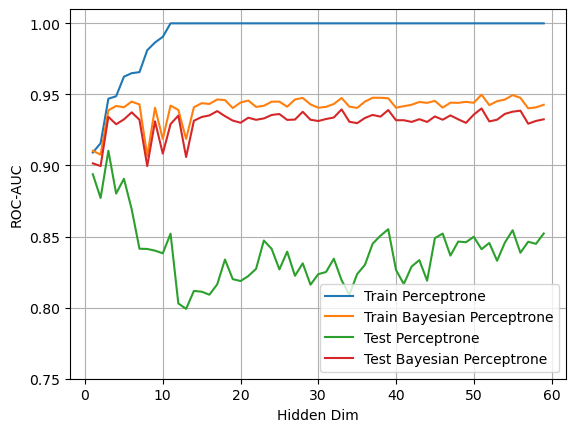
\includegraphics[width=1\linewidth]{roc_auc.png}
    \caption{Зависимость ROC--AUC от размерности скрытого состояния на тренировочных и тестовых данных}
    \label{fig:enter-label}
\end{figure}

\section{Выводы}
По результатам работы можно сделать следующие выводы:
\begin{itemize}
    \item с ростом сложности модели байесовская нейронная сеть не переобучилась;
    \item значение ROC-AUC на тестовой выборке имеет очень высокую корреляцию со значением ROC-AUC на тренировочной выборке (0.97 по Пирсону). Следовательно, для подбора гиперпараметров можно ориентироваться на метрики, полученные по тренировочной выборке. Это даёт нам возможность отказаться от деления на тренировочную и валидационную выборки для подбора гиперпараметров.
\end{itemize}

Так же стоит отметить, что данный подход переносится на другие архитектуры нейронных сетей (рекуррентные, свёрточные, трансформеры).

Имплементация данного подхода была выполнена с использованием PyTorch. Весь исходный код для проведения экспериментов размещён по адресу \url{https://github.com/dimabasow/bayesian-neural-networks}.

\end{document}
